\chapter{Electromagnetic radiation}\fancyfoot[LO,RE]{Physics: Waves, Sound and Light}
    \setcounter{figure}{1}
    \setcounter{subfigure}{1}
    \label{459e2bef85baf867f5850bc8338cad3a}
         \section{What is \textsl{electromagnetic radiation}?}
    \nopagebreak
%            \label{m38777} $ \hspace{-5pt}\begin{array}{cccccccccccc}   
\includegraphics[width=0.75cm]{col11305.imgs/summary_fullmarks.png} &   \end{array} $ \hspace{2 pt}\raisebox{-5 pt}{} {(section shortcode: P10050 )} \par 
  The most common example of electromagnetic (EM) radiation is visible light. Everyone is very familiar with light in everyday life, you can only see things because light bounces off them and enters your eyes. This alone makes it worthwhile to learn about it but there are also very many other applications of EM radiation. It is called electromagnetic because there are electric and magnetic fields making up the radiation. We will look at this in more detail a little later.

  In everyday experience, light doesn't seem to have many special properties but it does:
\begin{itemize}
 \item \textbf{A huge spectrum}: The light we can see (visible EM radiation) is only a small part of all of the EM radiation (electromagnetic spectrum) that exists.
 \item \textbf{Nature's speed limit}: Nothing moves faster than the speed of light. 
 \item \textbf{Wave nature}: All EM radiation has the ability to behave like a \texbf{wave} which we call wave-like behaviour.
 \item \textbf{Particle nature}: All EM radiation has the ability to behave like a \texbf{particle} which we call particle-like behaviour.
 \item \textbf{No medium required}: EM radiation can propagate without a medium through which to move even though they are waves.
\end{itemize}

Two important things to notice, we have mentioned:
\begin{enumerate}[noitemsep, label=\textbf{\arabic*}. ]
 \item waves without a medium and
 \item being both a particle and a wave.
\end{enumerate}
We will discuss this in the following sections and in even more detail in Grades 11 and 12.

    \label{m38777*cid3}
            \section{Wave-like nature of EM radiation}
            \nopagebreak
      \label{m38777*id186686}If you watch a colony of ants walking up the wall, they look like a thin continuous black line. But as you look closer, you see that the line is made up of thousands of separated black ants.\par 
      \label{m38777*id187029}Light and all other types of electromagnetic radiation seem like a continuous wave at first, but when one performs experiments with light, one can notice that light can have both wave- and particle-like properties. Just like the individual ants, light can also be made up of individual bundles of energy, or quanta of light.\par 
      \label{m38777*id187035}Light has both wave-like and particle-like properties (wave--particle duality), but only shows one or the other, depending on the kind of experiment we perform. A wave-type experiment shows the wave nature, and a particle-type experiment shows particle nature. One \textbf{cannot} test the wave and the particle nature at the same time. A particle of light is called a photon.\par 




\label{m38777*fhsst!!!underscore!!!id75}\Definition{Photon} {A photon is a quantum (energy packet) of light.} 


%       \label{m38777*id187062}The particle nature of light can be demonstrated by the interaction of photons with matter. One way in which light interacts with matter is via the photoelectric effect, which will be studied in detail in Chapter~.\par 
\label{m38777*secfhsst!!!underscore!!!id79}
%             \subsubsection*{Particle/wave nature of electromagnetic radiation}
%             \nopagebreak
%       \label{m38777*id187078}\begin{enumerate}[noitemsep, label=\textbf{\arabic*}. ] 
%             \label{m38777*uid1}\item Give examples of the behaviour of EM radiation which can best be explained using a wave model.\newline
% \label{m38777*uid2}\item Give examples of the behaviour of EM radiation which can best be explained using a particle model.\newline
% \end{enumerate}
%     \label{m38777*cid4}
% \par \practiceinfo
%  \par \begin{tabular}[h]{cccccc}
%  (1.) 004n  &  (2.) 004p  & \end{tabular}

            \subsection*{Fields}
            \nopagebreak
      \label{m38777*id187125}\textit{Accelerating charges} emit electromagnetic waves. A changing electric field generates a magnetic field and a changing magnetic field generates an electric field. This is the principle behind the propagation of electromagnetic waves, because electromagnetic waves, unlike sound waves, do not need a medium to travel through. 

EM waves propagate when an electric field oscillating in one plane produces a magnetic field oscillating in a plane at right angles to it, which produces an oscillating electric field, and so on. The propagation of electromagnetic waves can be described as \textsl{mutual induction}. The changing electric field is responsible for inducing the magnetic field and vice versa.\par We use $E$ to denote electric fields and $B$ to denote magnetic fields.\par
      \label{m38777*id187138}These mutually regenerating fields, most commonly described as \textsf{self-propagating}, travel through empty space at a constant speed of approximately $3\ensuremath{\times}{10}^{8}\phantom{\rule{0.166667em}{0ex}}\text{m}\ensuremath{\cdot}{\text{s}}^{-1}$, represented by $c$. We will use $3\ensuremath{\times}{10}^{8}\phantom{\rule{0.166667em}{0ex}}\text{m}\ensuremath{\cdot}{\text{s}}^{-1}$ for all of our calculations in this book.
      \label{m38777*eip-43}Although an electromagnetic wave can travel through empty space, it can also travel through a medium (such as water and air). When an electromagnetic wave travels through a medium, it travels slower than it would through empty space (vacuum).\par \label{m38777*id187191}
    \setcounter{subfigure}{0}
	\begin{figure}[H] % horizontal\label{m38777*id187194}
    \begin{center}

\begin{pspicture}(-4,-4)(3,4)
\psset{Alpha=30}
\pstThreeDCoor[nameY=$B$,nameZ=$E$,linecolor=black,xMin=-4,yMin=-4,zMin=-4]
\parametricplotThreeD[xPlotpoints=200,linecolor=blue,linewidth=1.5pt,plotstyle=curve,linestyle=dashed](-180,180){%
    t 60 div
    3 2.5 t mul cos mul
    0}
\parametricplotThreeD[xPlotpoints=200,linecolor=red,linewidth=1.5pt,plotstyle=curve](-180,180){%
    t 60 div
    0
     -3 2.5 t mul cos mul
    }
\end{pspicture}
\caption{
 A diagram showing the mutually regenerating electric field (red (solid) line) and magnetic field (blue (dashed) line).
}

 \end{center}
 \end{figure}       
      \par \label{m38777*eip-808}Since an EM radiation is a wave, the following equation still applies:\par \label{m38777*eip-181}\nopagebreak\noindent{}
    \begin{equation*}
    v=f\ensuremath{\cdot}\lambda
      \end{equation*}
      \label{m38777*eip-601}Except that we can replace $v$ with $c$:\par \label{m38777*eip-194}\nopagebreak\noindent{}
    \begin{equation*}
    \boxed{c=f\ensuremath{\cdot}\lambda}
      \end{equation*}
      \par
            \label{m38777*eip-923}
      \noindent
      \begin{wex}{EM radiation I}{
      \label{m38777*id187899}Calculate the frequency of an electromagnetic wave with a wavelength of $4,2\ensuremath{\times}{10}^{-7}$ m.}
      { 
      \westep{Wave equation}
      \label{m38777*id187948}We use the formula: $c=f\lambda $ to calculate frequency. The speed of light is a constant $3\ensuremath{\times}{10}^{8}~\text{m}\cdot\text{s}^{-1}$.\par 
      \westep{Calculate}  
    \begin{equation*}
    \begin{array}{ccc}\hfill c& =& f\lambda \hfill \\ \hfill 3\ensuremath{\times}{10}^{8}~\text{m}\cdot\text{s}^{-1}& =& f\ensuremath{\times}4,2\ensuremath{\times}{10}^{-7}~m\hfill \\ \hfill f& =& 7,14\ensuremath{\times}{10}^{14}\text{Hz}\hfill \end{array}
      \end{equation*}
\westep{Quote the final answer}
The frequency is $7,14\ensuremath{\times}{10}^{14}\text{Hz}$.}   \end{wex}
 
      \begin{wex}{EM Radiation II}{
      \label{m38777*id188123}An electromagnetic wave has a wavelength of $200\phantom{\rule{3.33333pt}{0ex}}\text{nm}$. What is the frequency of the radiation?}{
      \westep{What do we know?}
      \label{m38777*id188341}Recall that all radiation travels at the speed of light ($c$) in vacuum.
Since the question does not specify through what type of material the wave
is traveling, one can assume that it is traveling through a vacuum.
We can identify two properties of the radiation - $wavelength\phantom{\rule{3.33333pt}{0ex}}\left(200\phantom{\rule{3.33333pt}{0ex}}\text{nm}\right)$ and speed ($c$).\par 
    \westep{Apply the wave equation} 
    \begin{equation*}
    \begin{array}{ccc}\hfill c& =& f\lambda \hfill \\ \hfill 3\ensuremath{\times}{10}^{8}~\text{m}\cdot\text{s}^{-1}& =& f\ensuremath{\times}200\ensuremath{\times}{10}^{-9}~m\hfill \\ \hfill f& =& 1.5\ensuremath{\times}{10}^{15}\phantom{\rule{4pt}{0ex}}\text{Hz}\hfill \end{array}
      \end{equation*}
\westep{Quote the final answer}
The frequency is $1.5\ensuremath{\times}{10}^{15}\phantom{\rule{4pt}{0ex}}\text{Hz}$.
}    \end{wex}
         \section{Electromagnetic spectrum}
    \nopagebreak
%\label{m38778} $ \hspace{-5pt}\begin{array}{cccccccccccc}   
\includegraphics[width=0.75cm]{col11305.imgs/summary_fullmarks.png} &   \end{array} $ \hspace{2 pt}\raisebox{-5 pt}{} {(section shortcode: P10051 )} \par 
            \nopagebreak
EM radiation is classified into types according to the frequency of the wave: these types include, in order of increasing frequency, radio waves, microwaves, infrared radiation, visible light, ultraviolet radiation, X-rays and gamma rays.\par 
            \nopagebreak
      
      \label{m38778*id187332}Table~\ref{table:EMSpectrumRanges} lists the wavelength and frequency ranges of the divisions of the electromagnetic spectrum.\par 
    % \textbf{m38778*uid8}\par
          \begin{table}[H]
    % \begin{table}[H]
    % \\ '' '0'
        \begin{center}
      \label{m38778*uid8}
    \noindent
    
      \begin{tabular}[t]{|l|l|l|}\hline
                \textbf{Category}
               &
                \textbf{Range of Wavelengths (nm)}
               &
                \textbf{Range of Frequencies (Hz)}
              % make-rowspan-placeholders
     \tabularnewline\cline{1-1}\cline{2-2}\cline{3-3}
      %--------------------------------------------------------------------
        gamma rays &
        $\lessthan{}$1 &
                $\greatthan{}3\ensuremath{\times}{10}^{19}$
              % make-rowspan-placeholders
     \tabularnewline\cline{1-1}\cline{2-2}\cline{3-3}
      %--------------------------------------------------------------------
        X-rays &
        1-10 &
        $3\ensuremath{\times}{10}^{17}$-$3\ensuremath{\times}{10}^{19}$% make-rowspan-placeholders
     \tabularnewline\cline{1-1}\cline{2-2}\cline{3-3}
      %--------------------------------------------------------------------
        ultraviolet light &
        10-400 &
        $7,5\ensuremath{\times}{10}^{14}$-$3\ensuremath{\times}{10}^{17}$% make-rowspan-placeholders
     \tabularnewline\cline{1-1}\cline{2-2}\cline{3-3}
      %--------------------------------------------------------------------
        visible light &
        400-700 &
        $4,3\ensuremath{\times}{10}^{14}$-$7,5\ensuremath{\times}{10}^{14}$% make-rowspan-placeholders
     \tabularnewline\cline{1-1}\cline{2-2}\cline{3-3}
      %--------------------------------------------------------------------
        infrared &
        700-${10}^{5}$ &
        $3\ensuremath{\times}{10}^{12}$-$4,3\ensuremath{\times}{10}^{19}$% make-rowspan-placeholders
     \tabularnewline\cline{1-1}\cline{2-2}\cline{3-3}
      %--------------------------------------------------------------------
        microwave &
                ${10}^{5}-{10}^{8}$
               &
        $3\ensuremath{\times}{10}^{9}$-$3\ensuremath{\times}{10}^{12}$% make-rowspan-placeholders
     \tabularnewline\cline{1-1}\cline{2-2}\cline{3-3}
      %--------------------------------------------------------------------
        radio waves &
                $\greatthan{}{10}^{8}$
               &
                $\lessthan{}3\ensuremath{\times}{10}^{9}$
              % make-rowspan-placeholders
     \tabularnewline\cline{1-1}\cline{2-2}\cline{3-3}
      %--------------------------------------------------------------------
    \end{tabular}
      \end{center}
    \label{table:EMSpectrumRanges}
    \caption{Electromagnetic spectrum}
\end{table}
    \par
      \label{m38778*id188548}Examples of some uses of electromagnetic waves are shown in Table~\ref{Table:EMUses}.\par 
    % \textbf{m38778*uid9}\par
          \begin{table}[H]
    % \begin{table}[H]
    % \\ '' '0'
        \begin{center}
      \label{m38778*uid9}
    \noindent
    
      \begin{tabular}{|l|l|}\hline
                \textbf{Category}
               &
                \textbf{Uses}
              \\ \hline
        gamma rays &
        used to kill the bacteria in marshmallows and to sterilise medical equipment \\ \hline
        X-rays &
        used to image bone structures \\ \hline
        ultraviolet light &
        bees can see into the ultraviolet because flowers stand out more clearly at this frequency \\ \hline
        visible light &
        used by humans to observe the world \\ \hline
        infrared &
        night vision, heat sensors, laser metal cutting \\ \hline
        microwave &
        microwave ovens, radar \\ \hline
        radio waves &
        radio, television broadcasts \\ \hline
    \end{tabular}
      \end{center}\label{Table:EMUses}
        \caption{
	  Uses of EM waves
	}
\end{table}
\begin{exercises}{EM radiation}
            \nopagebreak
      \label{m38778*id188768}\begin{enumerate}[noitemsep, label=\textbf{\arabic*}. ] 
            \label{m38778*uid10}\item Arrange the following types of EM radiation in order of increasing frequency: infrared, X-rays, ultraviolet, visible, gamma.\newline
\label{m38778*uid11}\item Calculate the frequency of an EM wave with a wavelength of 400~nm.\newline
\label{m38778*uid12}\item Give an example of the use of each type of EM radiation, i.e. gamma rays, X-rays, ultraviolet light, visible light, infrared, microwave and radio and TV waves.\newline
\end{enumerate}
    \label{m38778*cid6}
\par \practiceinfo
 \par \begin{tabular}[h]{cccccc}
 (1.) 004q  &  (2.) 004r  &  (3.) 004s  & \end{tabular}
\end{exercises}
	\begin{figure}[H] % horizontal\label{m38778*uid3}
    \begin{center}
    \rule[.1in]{\figurerulewidth}{.005in} \\
        \label{m38778*uid3!!!underscore!!!media}\label{m38778*uid3!!!underscore!!!printimage}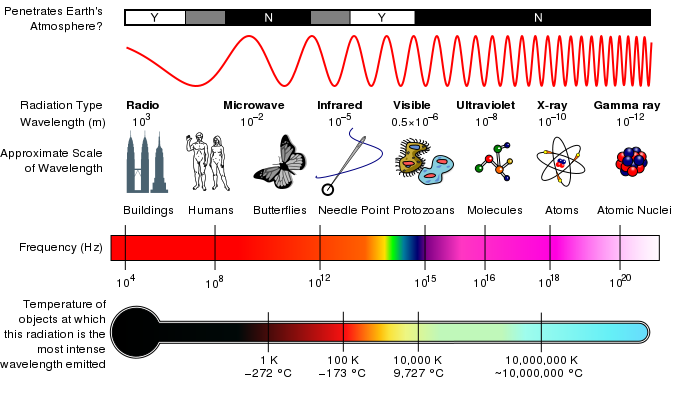
\includegraphics[width=\columnwidth]{col11305.imgs/m38778_EM_Spectrum_Properties_edit.png} % m38778;EM\_Spectrum\_Properties\_edit.png;;;6.0;8.5;
      \label{fig:emspectrum}
      \caption{The electromagnetic spectrum as a function of frequency. The different types according to wavelength are shown as well as everyday comparisons.
	}
    \rule[.1in]{\figurerulewidth}{.005in} \\
    \end{center}
 \end{figure}       
      \label{m38778*id187230}EM radiation in the visible part of the spectrum is scattered off all of the objects around us. This EM radiation provides the information to our eyes that allows us to see. The frequencies of radiation the human eye is sensitive to constitute only a very small part of all possible frequencies of EM radiation. The full set of EM radiation is called the electromagnetic spectrum. To simplify things the EM spectrum divided into sections (such as radio, microwave, infrared, visible, ultraviolet, X-rays and gamma-rays).\par 
      \label{m38778*eip-855}The EM spectrum is continuous (has no gaps) and infinite. Due to technological limitations, we can only use electromagnetic radiation with wavelengths between ${10}^{-14}\text{m}$ and ${10}^{15}\text{m}$.
\label{m38778*secfhsst!!!underscore!!!id117}
           \section{Penetrating ability of EM radiation}
            \nopagebreak
      \label{m38779*id189450}Different frequencies of EM radiation have different degrees of penetration. For example, if we take the human body as the object, visible light is reflected off the surface of the human body, ultra-violet light (from sunlight) damages the skin, but X-rays are able to penetrate the skin and bone and allow for pictures of the inside of the human body to be taken.\par 
      \label{m38779*id189457}If we compare the energy of visible light to the energy of X-rays, we find that X-rays have a much higher frequency. Usually, electromagnetic radiation with higher frequency (energy) have a higher degree of penetration than those with low frequency.\par 
      \label{m38779*id189462}Certain kinds of electromagnetic radiation such as ultra-violet radiation, X-rays and gamma rays are very dangerous. Radiation such as these are called ionising radiation. Ionising radiation transfers energy as it passes through matter, breaking molecular bonds and creating ions.\par 
      \label{m38779*id189468}Excessive exposure to radiation, including sunlight, X-rays and all nuclear radiation, can cause destruction of biological tissue. Luckily, the Earth's atmosphere protects us and other living beings on Earth from most of the harmful EM radiation.\par 
      \label{m38779*uid17}
            \subsubsection*{Ultraviolet (UV) radiation and the skin}
            \nopagebreak
        \label{m38779*id189482}UVA and UVB are different ranges of frequencies for ultraviolet (UV) light. UVA and UVB can damage collagen fibres which results in the speeding up skin aging. In general, UVA is the least harmful, but it can contribute to the aging of skin, DNA damage and possibly skin cancer. It penetrates deeply and does not cause sunburn. \par 
        \label{m38779*id189490}UVB light can cause skin cancer. The radiation excites DNA molecules in skin cells, resulting in possible cancerous mutations. In particular, the layer of ozone in the atmosphere protects us from UVB radiation. The connection between UVB radiation and cancer is one of the reasons for concern about the depletion of ozone in the atmosphere.\par 
        
\label{m38779*id189495}As a defense against UV radiation, the body tans when exposed to moderate (depending on skin type) levels of radiation by releasing the brown pigment melanin. This helps to block UV penetration and prevent damage to the vulnerable skin tissue deeper down. Sun-tan lotion, often referred to as sunblock or sunscreen, partly blocks UV radiation and is widely available. These products have a sun protection factor (SPF) rating (usually indicated on the container) that indicate how much protection the product provides against UVB radiation. The SPF rating does not specify protection against UVA radiation. Some sunscreen lotion now includes compounds such as titanium dioxide which helps protect against UVA rays. Other UVA-blocking compounds found in sunscreen include zinc oxide and avobenzone.\par 
\label{m38779*secfhsst!!!underscore!!!id701}
\begin{minipage}{.5\textwidth}
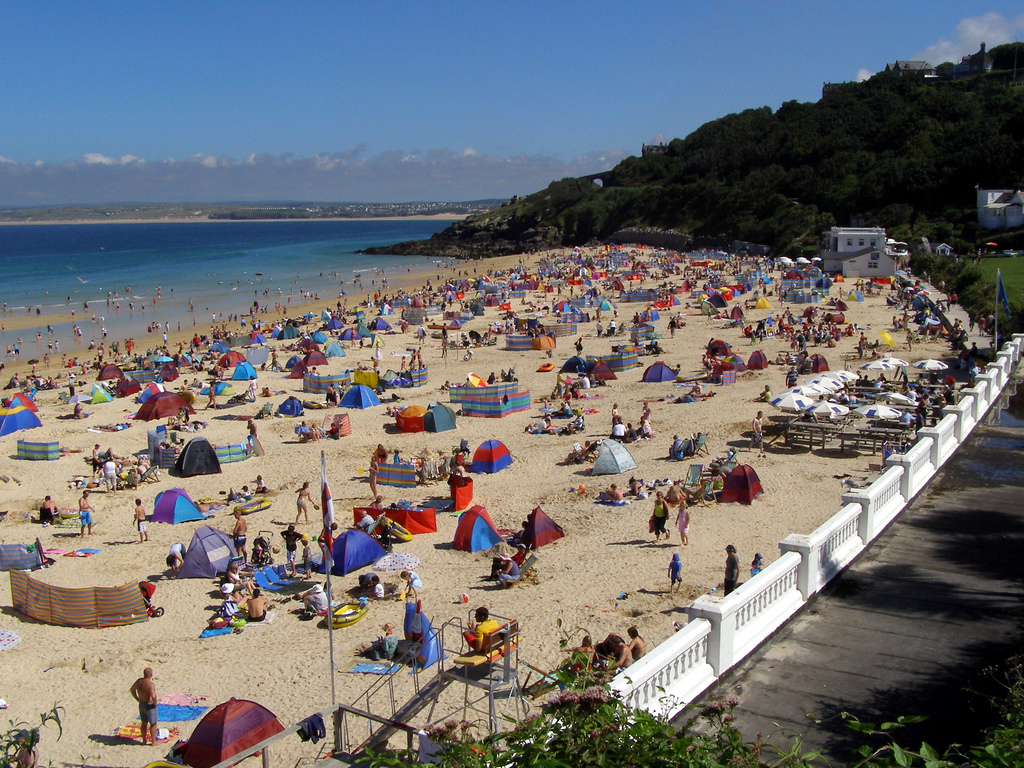
\includegraphics[width=.8\columnwidth]{photos/beach2_treehouse1977.jpg}
\end{minipage}
\begin{minipage}{.5\textwidth}
            \subsubsection*{What makes a good sunscreen? }
            \nopagebreak
        \label{m38779*id189518}\begin{itemize}[noitemsep]
            \label{m38779*uid18}\item UVB protection: Padimate O, Homosalate, Octisalate (octyl salicylate), Octinoxate (octyl methoxycinnamate)
\label{m38779*uid19}\item UVA protection: Avobenzone
\label{m38779*uid20}\item UVA/UVB protection: Octocrylene, titanium dioxide, zinc oxide, Mexoryl (ecamsule)
\end{itemize}
        \label{m38779*id189561}Another means to block UV is by wearing sun protective clothing. This is clothing that has a UPF rating that describes the protection given against both UVA and UVB. \par 
      \label{m38779*uid21}
\end{minipage}
            \subsubsection*{Ultraviolet radiation and the eyes}
            \nopagebreak
        \label{m38779*id189581}High intensity UVB light can cause damage to the eyes and exposure can cause welder's flash (photo keratitis or arc eye) and may lead to cataracts and other medical issues.\par 
        \label{m38779*id189586}Protective eyewear is beneficial to those who are working with or those who might be exposed to ultraviolet radiation. Given that light may reach the eye from the sides, full coverage eye protection is best.
        \label{m38779*id189594}Ordinary, untreated glasses give some protection. Most plastic lenses give more protection than glass lenses. Some plastic lens materials, such as polycarbonate, block most UV. Most contact lenses help to protect the retina by absorbing UV radiation.\par 
      \label{m38779*uid22}
\begin{minipage}{.5\textwidth}
            \subsubsection*{X-rays}
            \nopagebreak
        \label{m38779*id189613}While X-rays are used significantly in medicine, prolonged exposure to X-rays can lead to cell damage and cancer.\par 
        \label{m38779*id189617}For example, a mammogram is an X-ray of the human breast to detect breast cancer, but if a woman starts having regular mammograms when she is too young, her chances of getting breast cancer increases.\\
      \label{m38779*uid23}

            \subsubsection*{Gamma-rays}
            \nopagebreak
        \label{m38779*id189632}Due to their high energies, gamma-rays are able to cause serious damage when absorbed by living cells.\par 
        \label{m38779*id189636}Gamma-rays are not stopped by the skin and can induce DNA alteration by interfering with the genetic material of the cell. DNA double-strand breaks are generally accepted to be the most biologically significant lesion by which ionising radiation causes cancer and hereditary disease.\par 
        \label{m38779*id189642}A study done on Russian nuclear workers exposed to external whole-body gamma-radiation at high doses shows a link between radiation exposure and death from leukaemia, lung, liver, skeletal and other solid cancers.\par 
      \label{m38779*eip-665}
\end{minipage}
\begin{minipage}{.5\textwidth}\begin{center}
 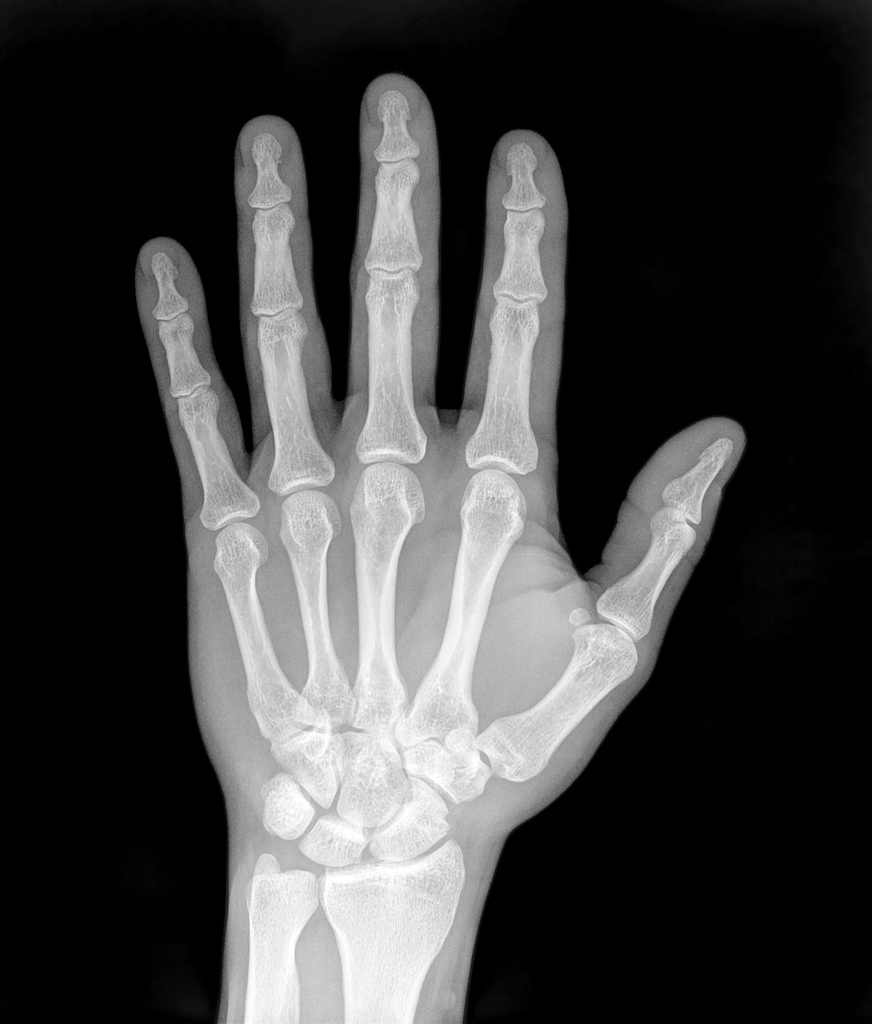
\includegraphics[width=0.8\textwidth]{photos/x-ray-hand_TraceMeek_flickr.jpg}\end{center}
\end{minipage}

            \subsubsection*{Cellphones and microwave radiation}
            \nopagebreak
\begin{minipage}{.5\textwidth}
\includegraphics[width=.8\columnwidth]{photos/cellphones_kapungo.jpg}
\end{minipage}
\begin{minipage}{.5\textwidth}
            \label{m38779*id189654}Cellphone radiation and health concerns have been raised, especially following the enormous increase in their use. This is because cellphones use electromagnetic waves in the microwave range. These concerns have induced a large body of research. Concerns about effects on health have also been raised regarding other digital wireless systems, such as data communication networks.
In 2009 the World Health Organisation announced that they have found a link between brain cancer and cellphones. However, there is still no firm evidence for this and the link is tenuous at best. You can find out more at http://www.who.int/mediacentre/factsheets/fs193/en/\footnote{http://www.who.int/mediacentre/factsheets/fs193/en/}
        \par 
\end{minipage}
        \label{m38779*id189664}Cellphone users are recommended to minimise their exposure to the radiation, by for example:\par 
        \label{m38779*id189668}\begin{enumerate}[noitemsep, label=\textbf{\arabic*}. ] 
            \label{m38779*uid24}\item Use hands-free to decrease the radiation to the head.
\label{m38779*uid25}\item Keep the mobile phone away from the body.
\label{m38779*uid26}\item Do not use a cellphone in a car without an external antenna.
\end{enumerate}
        \label{m38779*uid27}
            \begin{exercises}{Penetrating ability of EM radiation}
            \nopagebreak
        \label{m38779*id189729}\begin{enumerate}[noitemsep, label=\textbf{\arabic*}. ] 
            \label{m38779*uid28}\item Indicate the penetrating ability of the different kinds of EM radiation and relate it to energy of the radiation.\newline
\label{m38779*uid29}\item Describe the dangers of gamma rays, X-rays and the damaging effect of ultra-violet radiation on skin.\newline
\end{enumerate}
    \label{m38779*cid8}
% \par \practiceinfo
 \par \begin{tabular}[h]{cccccc}
 (1.) 004t  &  (2.) 004u  &  \end{tabular}
\end{exercises}


            \section{Particle-like nature of EM radiation}
            \nopagebreak
      \label{m38778*id188832}When we talk of electromagnetic radiation as a particle, we refer to photons, which are packets of energy. The energy of the photon is related to the wavelength of electromagnetic radiation according to:\par 
\Definition{Planck's constant} {Planck's constant is a physical constant named after Max Planck.\\ $h=6,63\ensuremath{\times}{10}^{-34}$ J $\ensuremath{\cdot}$ s} 
      \label{m38778*id188898}The energy of a photon can be calculated using the formula: 
\begin{equation*}
\boxed{E=hf}
\end{equation*} 
or 
\begin{equation*}
\boxed{E=h\frac{c}{\lambda}},
\end{equation*}where E is the energy of the photon in joules (J), $h$ is Planck's constant, $c$ is the speed of light, $f$ is the frequency in hertz (Hz) and $\lambda $ is the wavelength in metres (m).\par The higher the frequency of EM radiation, the higher the energy. 
      \begin{wex}{Calculating the energy of a photon I}{
      \label{m38778*id188962}Calculate the energy of a photon with a frequency of $3\ensuremath{\times}{10}^{18}$~Hz}{
\westep{Analyse the question}
You are asked to determine the energy of a photon given the frequency. The frequency is in standard units and we know the relationship between frequency and energy.
  \westep{Apply the equation for the energy of a photon}
    \begin{eqnarray}
    E& =& hf\\ 
     & =& 6,63\ensuremath{\times}{10}^{-34}~\text{J}\cdot\text{s}\ensuremath{\times}3\ensuremath{\times}{10}^{18}~\text{Hz}\\ 
     & =& 2\ensuremath{\times}{10}^{-15}\phantom{\rule{0.166667em}{0ex}}\text{J}
      \end{eqnarray}
  \westep{Quote the final result}
  The energy is $2\times{10}^{-15}$~J}\end{wex}
    
  \begin{wex}{Calculating the energy of a photon II}{What is the energy of an ultraviolet photon with a wavelength of 200~nm?}{
\westep{Analyse the question}
You are asked to determine the energy of a photon given the wavelength. The wavelength is in standard units and we know the relationship between frequency and energy. We also know the relationship between wavelength and frequency, the equation for wave speed. The speed of light is a constant that we know.
   \westep{Apply principles}
First we determine the frequency in terms of the wavelength.
\begin{align*}
 c&=f\cdot\lambda\\
 f&=\frac{c}{\lambda}
\end{align*}
We can substitute this into the equation for the energy of a photon, $E=hf$, allowing us to deduce:
    \begin{equation*}
    E=h\frac{c}{\lambda }
      \end{equation*}
      \label{m38778*id189220}\nopagebreak\noindent{}
 \westep{Do the calculation}   
    \begin{equation*}
    \begin{array}{ccc}\hfill E& =& h\frac{c}{\lambda }\hfill \\ & =& \left(6,63\ensuremath{\times}{10}^{-34}~\text{J}\cdot\text{s}\right)\frac{3\ensuremath{\times}{10}^{8}\text{m}\cdot\text{s}^{-1}}{200\ensuremath{\times}{10}^{-9}~\text{m}}\hfill \\ & =& 9,939\ensuremath{\times}{10}^{-10}\phantom{\rule{0.166667em}{0ex}}\text{J}\hfill \end{array}
      \end{equation*}
\westep{Quote the final result}
The energy of the photon is $9,939\ensuremath{\times}{10}^{-10}\phantom{\rule{0.166667em}{0ex}}\text{J}$}
         \end{wex}
      \label{m38778*uid13}
            \begin{exercises}{Particle nature of EM waves}
            \nopagebreak
        \label{m38778*id189384}\begin{enumerate}[noitemsep, label=\textbf{\arabic*}. ] 
            \label{m38778*uid14}\item How is the energy of a photon related to its frequency and wavelength?\newline
\label{m38778*uid15}\item Calculate the energy of a photon of EM radiation with a frequency of ${10}^{12}$~Hz.\newline
\label{m38778*uid16}\item Determine the energy of a photon of EM radiation with a wavelength of 600 nm.\newline
\end{enumerate}
  \label{m38778**end}
\par \practiceinfo
 \par \begin{tabular}[h]{cccccc}
 (1.) 004v  &  (2.) 004w  &  (3.) 004x  & \end{tabular}
\end{exercises}
            
    \label{m38779*eip-745}
            \subsection*{Animal behaviour}
            \nopagebreak
            \label{m38779*id1164126080746}People have believed that animals can predict earthquakes and other natural disasters for centuries. As early as 373 B.C., historians recorded a massive exodus of animals, including rats, snakes and weasels, from the Greek city of Helice days before a quake struck causing massive devastation.\par 
      \label{m38779*id1164126439136}This topic is much debated and different behaviours are sometimes seen for different kinds of animals, for example:\par 
      \label{m38779*id1164132827593}\begin{itemize}[noitemsep]
            \item \textbf{Dogs and cats}: are believed by pet owners to howl or bite their owners before natural disasters, they cite factors like a much stronger sense of smell.
\item \textbf{Sharks}: researchers in Florida have reported that sharks are observed to move to deeper water before hurricanes, possibly because of a sensitivity to changes in the air pressure preceding the hurricane.
\item \textbf{Rodents}: rodents that live underground will often flee their holes and burrows before a disaster. Scientists from the California Institute of Technology have noted that there are many changes preceding earthquakes such as tilting of the Earth. Rodents are often more sensitive to such small changes and will react to these changes.
\item \textbf{Elephants}: will allegedly trumpet and flee to higher ground before a tsunami arrived. This is attributed to their being more sensitive to vibrations on the Earth's surface. \end{itemize}
      \label{m38779*id1164121170251}Many researchers argue that animals detect certain natural signals, such as the early tremblings of an earthquake, long before humans. This means that the animals have opportunity to react before we can. However it can be said that they exhibit no special understanding, they just flee as would any person hearing a shout of fire.\par 
      \label{m38779*id6489198}Another problem cited with these seemingly clairvoyant animals is that their psychic powers often are based on behaviors that people only recall after the event. Some animal behaviors happen frequently, but are not remembered unless an earthquake, tsunami, or mud slide follows. For example, if you see a dog cross a road, you just remember you saw a dog cross the road. But if an earthquake shook your neighborhood five minutes later, would you say the dog was fleeing? \par 
      \label{m38779*id1553831}
            \begin{project}{Animals and natural disasters}
            \nopagebreak
        \label{m38779*id1164119615164}Carry out research on the behavior of animals before natural disasters. \par 
        \label{m38779*id1164121934705}Pick one type of natural disaster (earthquake, flood, tsunami, etc.) and see what you can find about animals reacting to that type of disaster. Ask people you know about what they have heard to get a sense of folklore.\par 
        \label{m38779*id1164121037612}Then research the topic to find more information and remember to critically assess all information. Things to consider:\par 
        \label{m38779*id1164128014077}\begin{itemize}[noitemsep]
            \item What scientific research has been conducted?  
\item Which countries does that type of disaster usually occur in?
\item Do any of the native people of that country have legends/ideas about animals reacting to the disaster? 
\item What do people believe leads to this behavior? i.e. do the animals have some mystic ability or are they more sensitive to anything then we are (such as low frequency radiation)\end{itemize}
Some suggested resources for information are: 
\begin{itemize}[noitemsep]
\item \textsl{http://www.unep.org/ik/}
\item \textsl{http://earthquake.usgs.gov/learn/topics/animal\_eqs.php}
\item \textsl{http://biology.about.com/od/animalbehavior/a/aa123104a.htm} 
\item \textsl{http://news.nationalgeographic.com/news/2003/11/1111\_031111\_earthquakeanimals\_2.html}
\item \textsl{Bats sing, mice giggle} by Karen Shanor and Jagmeet Kanwal
\item \textsl{http://www.sheldrake.org/homepage.html}
\item \textsl{http://nationalzoo.si.edu/SCBI/AnimalCare/News/earthquake.cfm}
\item \textsl{http://www.animalvoice.com/animalssixthsense.htm}
\end{itemize}
        \label{m38779*id1164121076422}Present your findings to your class. Critically analyze all the information you collect and decide what you believe. \par 
      \label{m38779*cid9}
      \end{project}

\summary{Placeholder}
            \nopagebreak
      \label{m38779*id189769}\begin{enumerate}[noitemsep, label=\textbf{\arabic*}. ] 
            \label{m38779*uid30}\item Electromagnetic radiation has both a wave and a particle nature.
\label{m38779*uid31}\item Electromagnetic waves travel at a speed of approximately $3\ensuremath{\times}{10}^{8}\phantom{\rule{3.33333pt}{0ex}}m\ensuremath{\cdot}{s}^{-1}$ in a vacuum.
\label{m38779*uid32}\item The Electromagnetic spectrum consists of the following types of radiation: radio waves, microwaves, infrared, visible, ultraviolet, X-rays, gamma-rays.
\label{m38779*uid33}\item Gamma-rays have the most energy and are the most penetrating, while radio waves have the lowest energy and are the least penetrating.
\end{enumerate}
\begin{table}[H]
\begin{center}
\begin{tabular}{|l|c|c|c|}\hline \hline 
\multicolumn{4}{|c|}{\textbf{Units}}\\ \hline \hline
\textbf{Quantity} & \textbf{Symbol} & \textbf{Unit} & \textbf{S.I. Units}\\ \hline
Energy & $E$ & J & $ \text{kg}\cdot\text{m}^2\cdot\text{s}^{−2}$ \\ \hline
Wavelength & $\lambda$ & \multicolumn{2}{c|}{m}  \\ \hline
Period & $T$ & \multicolumn{2}{c|}{s}  \\ \hline
Frequency & $f$ & Hz & $\text{s}^{-1}$  \\ \hline
Speed of light & $c$ & \multicolumn{2}{c|}{$\text{m} \cdot \text{s}^{-1}$} \\ \hline
\end{tabular}
\end{center}
\caption{Units used in \textbf{electromagnetic radiation} }
\label{table:electricity::units}
\end{table}
            \begin{eocexercises}{End of chapter exercise}
            \nopagebreak
      \label{m38779*id189872}\begin{enumerate}[noitemsep, label=\textbf{\arabic*}. ] 
            \label{m38779*uid34}\item What is the energy of a photon of EM radiation with a frequency of $3\ensuremath{\times}{10}^{8}$~Hz?\newline
\label{m38779*uid35}\item What is the energy of a photon of light with a wavelength of 660~nm?\newline
\label{m38779*uid36}\item List the main types of electromagnetic radiation in order of increasing wavelength.\newline
\label{m38779*uid37}\item List the main uses of:
\label{m38779*id189946}\begin{enumerate}[noitemsep, label=\textbf{\alph*}. ] 
            \label{m38779*uid38}\item radio waves
\label{m38779*uid39}\item infrared
\label{m38779*uid40}\item gamma rays
\label{m38779*uid41}\item X-rays
\end{enumerate}
                \label{m38779*uid42}\item Explain why we need to protect ourselves from ultraviolet radiation from the Sun.\newline
\label{m38779*uid43}\item List some advantages and disadvantages of using X-rays.\newline
\label{m38779*uid44}\item What precautions should we take when using cell phones?\newline
\label{m38779*uid45}\item Write a short essay on a type of electromagnetic waves. You should look at uses, advantages and disadvantages of your chosen radiation.\newline
\label{m38779*uid46}\item Explain why some types of electromagnetic radiation are more penetrating than others.\newline
\end{enumerate}
  \label{m38779**end}
  \label{459e2bef85baf867f5850bc8338cad3a**end}
\par \practiceinfo
 \par \begin{tabular}[h]{cccccc}
 (1.) 004y  &  (2.) 004z  &  (3.) 0050  &  (4.) 0051  &  (5.) 0052  &  (6.) 0053  &  (7.) 0054  &  (8.) 0055  &  (9.) 0056  & \end{tabular}
\end{eocexercises}
